\chapter{Introduction}\label{ch:intr}
The phenomena of heavy-tailedness is widely observed in many
disciplines of science, for example, phase transition of matter and
black body radiation as studied in physics, neuronal avalanches in
biology, claim sizes of insurance mathematics and stock returns in
finance. The last application is indeed the focus of this thesis. To
discuss the phenomena in precise terms, we introduce the concept of
regular variation.

\section{Regular Variation}\label{sec:intro_regvar}
The concept of regular variation is defined by the following scaling
property: if a function $f$ on $(0, \infty)$ satisfies
\[
\lim_{x \to \infty} {f(c x) \over f(x)} = c^\alpha
\quad
\forall c > 0,
\]
then we say $f$ is regularly varying with index $\alpha$.
$f$ can be written in the form $f(x) = {L(x) \over x^\alpha}$, where
$L(x)$ is a slowly varying function, i.e.
$\lim_{x \to \infty} {L(c x) \over L(x)} = 1$, $\forall c > 0$.
We call a random variable $X$ regularly varying with index
$\alpha \geq 0$ if it satisfies the tail balance condition in the
limit $x \to \infty$.
\[
\P(X > x) \sim p_+ {L(x) \over x^\alpha},\quad
\P(X < -x) \sim p_- {L(x) \over x^\alpha}, \quad
\text{for some } p_+, p_- > 0,\; p_+ + p_- = 1
\]

% Distribution functions, say $F(\cdot)$, whose survival function
% $\bar F(x) = 1 - F(x)$ satisfies the above scaling property, are
% observed in a variety of phenomena, 
When expanded to multiple dimensions, the scaling property of regular
variation is better described in terms of vague convergence to a
spectral measure $\mu_\alpha$: if a random vector $X$ satisfies
\[
{
  \P(X/|X| \in \cdot, |X| > c x)
  \over
  \P(|X| > x)
}
\overset{v}{\to} c^{-\alpha} \mu_\alpha(\cdot),
\quad
x \to \infty, \forall c > 0,
\]
then we say $X$ is regularly varying with index $\alpha$. Here
$\mu_\alpha$ is a probability measure on the unit sphere
\cite{buraczewski:damek:mikosch:2016}. It is called the spectral 
measure of $X$ and $\alpha$ is again the tail index.
If $X$ is regularly varying with index $\alpha$, then each component
and each linear combination of its components are regularly
varying with the same index $\alpha$. This follows from Feller
\cite{feller}, p. 278. Cf. also Jessen and Mikosch
\cite{JessenMikosch2006}, lemma 3.1, and Embrechts et. al.
\cite{embrechts:klueppelberg:mikosch:1997}, lemma 1.3.1.

Clearly, estimating the tail index $\alpha$ of a sequence
$X_1, X_2, \dots$ of regularly varying variables is particularly
important for understanding the behavior of a heavy-tailed series. A
standard method proposed for this purpose is due to Hill
\cite{hill1975simple}:
\begin{equation}
  \label{eq:fhhty}
  \hat \alpha_H = \left[
    {1 \over k} \sum_{i=1}^k \log \left(
      X_{(i)} \over X_{(k+1)}
    \right)
  \right]^{-1},
\end{equation}
where $X_1, X_2, \dots, X_n$ is a sample whose tail index is the
subject of estimation, and $X_{(i)}$ is the $i$-th upper order
statistic of the sample. Several authors have contributed to showing
the weak consistency and asymptotic normality of the estimator
$\hat \alpha_H$, under the assumptions $k \to \infty, k/n \to 0$
as $n \to \infty$. See theorem 6.4.6 of Embrechts et. al.
\cite{embrechts:klueppelberg:mikosch:1997} for details.

%% Mason \cite{mason:1982} first proved that the estimator
%% was consistent when $X_1, X_2, \dots$ were iid; later Rootz\'en,
%% Leadbetter and de Haan \cite{rootzen:leadbetter:dehaan1992} and Hsing
%% \cite{hsing:1991} proved its consistency when $X_1, X_2, \dots$ were
%% weakly dependent; and Resnick and St{\u a}ric{\u a}
%% \cite{resnick:starica:1995, resnick:starica:1997} proved its
%% consistency when $X_t$ was a linear process.

Figure \ref{fig:thjyuj} shows the Hill estimates of the tail indices
of daily stock return series from 3 sectors of the
{\em Standard \& Poor's 500} index\footnote{An American stock index
  comprising around 500 companies.}. The 2.5\% and 97.5\% quantiles of
the asymptotic normal distribution of the estimates are also
given. One can see the confidence bands are fairly large compared with
the estimated values. This certainly raises the question of how
similar they really are and if/how their variations can be explained by
economic arguments.

%% We explore this topic in chapter \ref{ch:TailParameters}.

\begin{figure}[htb!]
  \begin{minipage}{1.0\linewidth}
    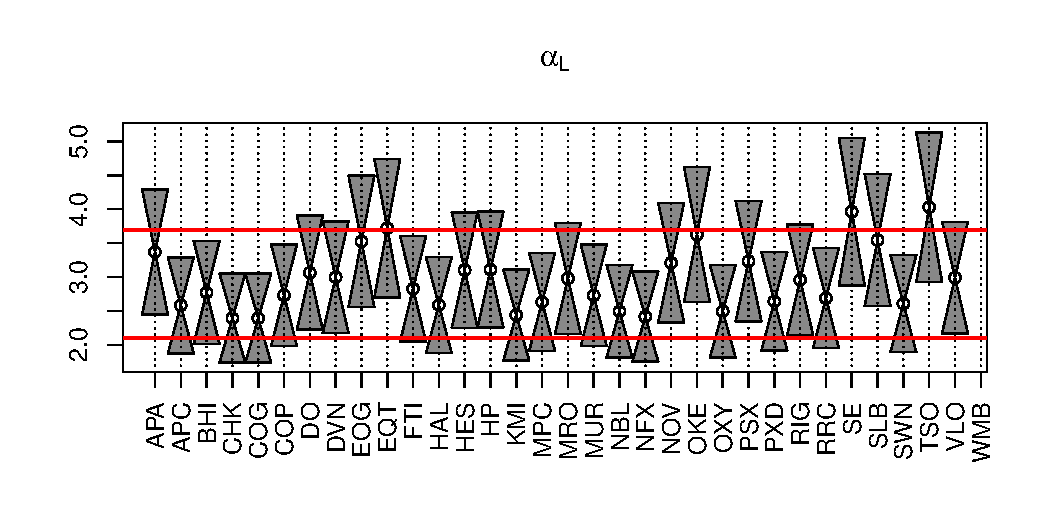
\includegraphics[width=\textwidth, trim={0, 0.8cm, 0, 2cm}, clip]
    {Energy_lower.pdf}
  \end{minipage}
  \begin{minipage}{1.0\linewidth}
    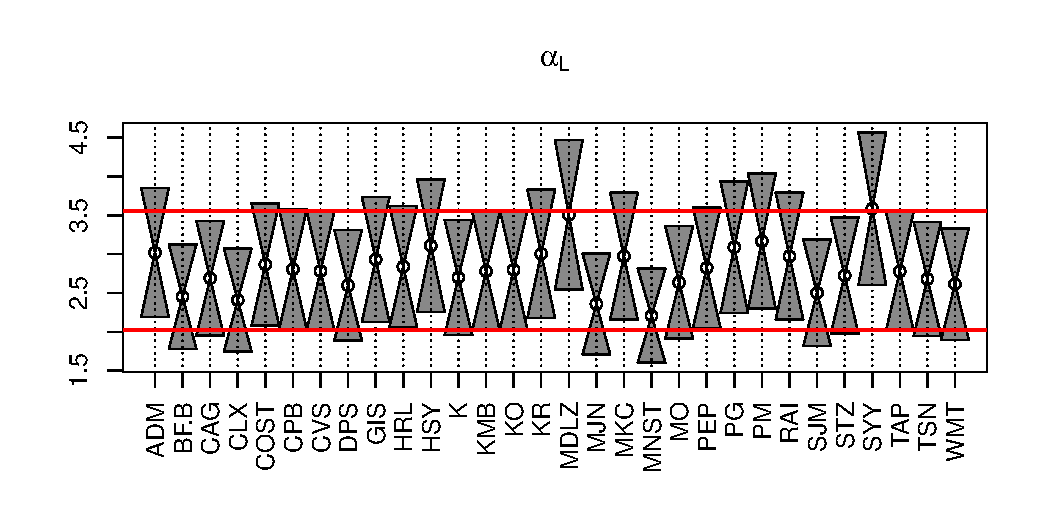
\includegraphics[width=\textwidth, trim={0, 0.8cm, 0, 2cm}, clip]
    {Consumer_Staples_lower.pdf}
  \end{minipage}
  \begin{minipage}{1.0\linewidth}
    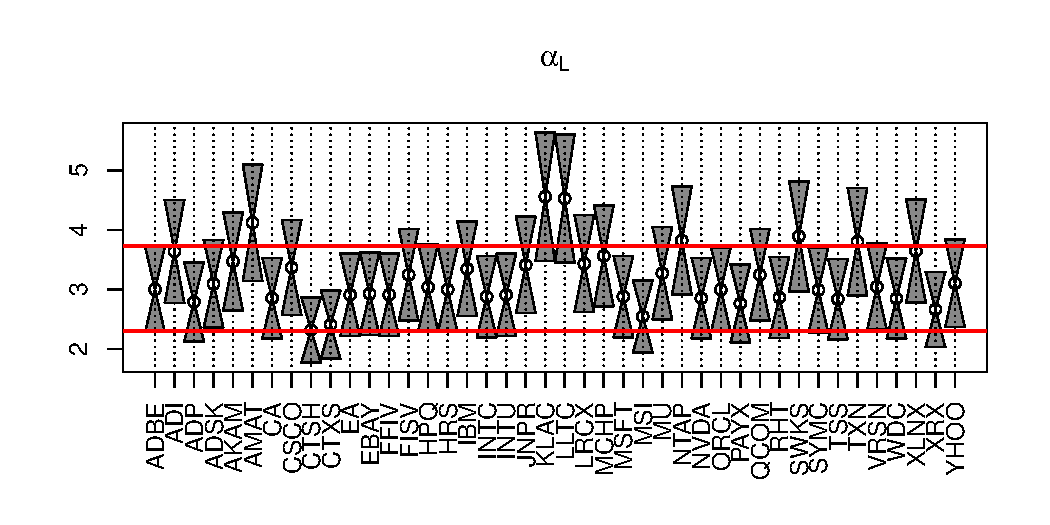
\includegraphics[width=\textwidth, trim={0, 0.8cm, 0, 2cm}, clip]
    {Information_Technology_lower.pdf}
  \end{minipage}
  \caption{\small Hill estimates $\hat \alpha_{50}$ of the lower
    tail-indices $\alpha$ of daily return series in sectors of the S\&P 500
    index. The data span from 1 January 2010 to 31 December 2014 and
    comprise $n=1304$ observations.
    The graphs from top to bottom correspond to the ``Energy'',
    ``Consumer Staples'' and ``Information Technology'' sectors.
    Each circle corresponds to a Hill estimate $\hat\alpha_{50}$; the gray
    triangles above and below it mark the 97.5\% and 2.5\% quantiles
    of its approximate normal distribution; see \eqref{eq:2} and the
    discussion following it for an interpretation.
    The lower and upper red lines mark the medians of the 2.5\% 
    and 97.5\% quantiles, respectively, evaluated from all stocks in
    the sector.
    The data are taken from {\it Yahoo Finance}; the labels on
    the horizontal axes are Yahoo symbols of the stocks. 
  }\label{fig:thjyuj}
\end{figure}

Random variables with regularly varying tails have some very nice
features: if $X_1$ and $X_2$ are both regularly varying with indices
$\alpha_1$ and $\alpha_2$, respectively, then $a_1 X_1 + a_2 X_2$,
for $a_1, a_2 > 0$, is regularly varying with index
$\min\{\alpha_1, \alpha_2\}$ (cf. Mikosch and Jessen
\cite{JessenMikosch2006}). Moreover, if $X_1, X_2$ are iid,
$\P(a_1 X_1 + a_2 X_2 > u) \sim \P(a_1 X_1 > u) + \P(a_2 X_2 > u)$.

Now consider $p$ return series
$X_{i,t}$, $i=1,2,\dots, p; t=1,\dots,n$.
Suppose each of these series is a linear combination of $K$ factors
$Y_{j,t}$, $j=1,2,\dots,K$, the $j$-th of which is regularly varying
with index $\alpha_j$. Then by the summation property, each and every
$\{X_{i,t}\}$ is regularly varying with index $\min_{1 \leq j \leq K} \alpha_j$.
In practice a factor $Y_{i,t}$ is estimated as
$\hat Y_{j,t} = \sum_{i=1}^p a_{j, i} X_{i,t}$, where
$(a_{j, 1}, a_{j, 2}, \dots, a_{j, p})^\top$ is the $j$-th eigenvector
of the sample covariance matrix of
$\{X_{i,t}\}, i=1,\dots,p; t=1,\dots,n$, i.e. the eigenvector
associated with the $j$-th largest eigenvalue. 
For this reason, it is important to understand the eigensystem of the
sample covariance matrix of $\{X_{i,t}\}$. This topic is addressed in
chapters \ref{ch:bernoulli} and \ref{ch:extremes} of this thesis.

When a product of independent positive random variables, say $X_1
X_2$, involves one with regularly varying tails, a useful result is
that of Breiman \cite{breiman:1965}: assume $X_1$ is regularly varying
with index $\alpha$ and there exists $\epsilon > 0$ such that
$\E X_2^{\alpha + \epsilon} < \infty$.
Then $\P(X_1 X_2 > x) \sim \E X_2^{\alpha} \P(X_1 > x)$.
More generally, if $X_1, X_2$ are regularly varying with the same tail
index $\alpha$ or if $\P(X_2 > x) = o(\P(X_1 > x))$, then $X_1 X_2$ is
regularly varying with index $\alpha$.

In addition to Breiman's result, the following is also well-known,
assuming $X_1, X_2$ are positive independent random variables and
$X_1$ is regularly varying with index $\alpha$:
\begin{enumerate}
\item if $X_2$ is regularly varying with index $\alpha$ or
  $\lim_{x \to \infty} {P(X_2 > x) \over \P(X_1 > x)} = 0$, then $X_1
  X_2$ is regularly varying with index $\alpha$.
\item if $X_1, X_2$ are iid and $\E X_1^\alpha = \infty$, then
  ${\P(X_1 X_2 > x) \over \P(X_1 > x)} \to \infty$
\item if $X_1, X_2$ are iid and $\E X_1^\alpha < \infty$, then the
  only possible limit of ${\P(X_1 X_2 > x) \over \P(X_1 > x)}$ is
  $2 \E X_1^\alpha$.
\end{enumerate}
For an extensive summary of the regular variation properties of
functions of regularly varying random variables, see Mikosch and
Jessen \cite{JessenMikosch2006}.

The notion of a regularly varying strictly stationary process is also of
interest. Originally introduced by Davis and Hsing
\cite{davis:hsing:1995} for univariate processes, the concept was
extended to multivariate processes by Davis and Mikosch
\cite{davis:mikosch:2009b}: An $\reals^d$-valued strictly stationary
process $X_t$ is said to be regularly varying with index $\alpha$, if
for each $h \geq 0$, 
\[
  {
    \P\left[x^{-1}(X_0, X_1, \dots, X_h) \in \cdot \right]
    \over
    \P(|X_0| > x)
  } \overset{v}{\to} \nu_\alpha(\cdot),
  \quad x \to \infty
\]
where $\nu_\alpha$ a non-null Radon measure on
$\reals^{d(h+1)} \setminus \{0\}$ that
is homogeneous of order $-\alpha$, i.e.
$\forall c > 0, \forall S \subset \reals^{d(h+1)}\setminus\{0\}, \nu_\alpha(c S) = c^{-\alpha} \nu_\alpha(S)$. $|\cdot|$ could be any given vector norm.

Basrak and Segers \cite{basrak:segers:2009} proved an equivalence
condition for regular variation of
a strictly stationary process: an $\reals^d$-valued strictly stationary
process $\{X_t\}$ is regularly varying with index $\alpha$ if 
there exists an $\reals^d$-valued sequence $\{\Theta_i\}_{i = 0,1,\ldots}$
and a Pareto($\alpha$) random variable $Z$, i.e.
$\P(Z > x) = x^{-\alpha}, \forall x \geq 1$, independent of
$\{\Theta_i\}$
\[
\P\left[\left.
  x^{-1}(X_0, X_1, \ldots) \in \cdot
  \right| |X_0| > x
  \right]
  \overset{w}{\to}
  \P(Z(\Theta_1, \Theta_2, \ldots) \in \cdot),
  \quad
  x \to \infty.
\]
The sequences $\{\Theta_i\}_{i = 0,1,\ldots}$ and
$\{Z \Theta_i\}_{i = 0,1,\ldots}$ are called the spectral tail process
and the tail process of $\{X_t\}$, respectively.

A recent remarkable result from Mikosch and Wintenberger
\cite{mikosch:wintenberger:2016} regarding
strictly stationary regularly varying processes is quoted below:
\begin{theorem}\label{thm:mikwin:intro}
Let $(Y_t)$ be an $\bbr^d$-valued strictly stationary sequence , $S_n=Y_1+\cdots +Y_n$ and $(a_n)$ be such that $n\,\P(|Y|>a_n)\to 1$.
Also write for $\vep>0$, $\ov Y_t = Y_t \I(|Y_t|\le \vep a_n)$, $\underline Y_t= Y_t-\ov  Y_t $ and
\beao
\ov S_{l,n}= \sum_{t=1}^l \ov Y_t \qquad  \un S_{l,n}= \sum_{t=1}^l \un Y_t\,.
\eeao
Assume the following conditions:
\begin{enumerate}
\item 
$(Y_t)$ is regularly varying with index $\alpha\in (0,2)  \setminus\{1\}$ and spectral tail process $(\Theta_j)$.
\item
A mixing condition holds: there exists an integer \seq\ $m_n\to\infty$ \st\ $k_n= [n/m_n]\to \infty$
and 
\beam\label{eq:chfa:intro}
\E \ex^{it'\underline S_n/a_n} - \Big(\E \ex^{it'\underline S_{m_n,n}/a_n}\Big)^{k_n} \to 0\,,\qquad \nto\,,\qquad t\in\bbr^d\,.
\eeam
\item An anti-clustering condition holds:
\beam\label{eq:acl:intro}
\lim_{l\to\infty} \limsup_{\nto} \P\big(\max_{t=l,\ldots,m_n} |Y_t|>\delta a_n\mid |Y_0|>\delta a_n\big)=0\,,\qquad \delta>0\,
\eeam
for the same sequence $(m_n)$ as in (2).
\item If $\alpha\in (1,2)$, in addition $\E[Y]=0$ and the vanishing small values condition holds: 
\beam\label{eq:vansm:intro}
\lim_{\vep\downarrow 0}\limsup_{\nto} \P\big(a_n^{-1} |\ov S_n-\E [\ov S_n]|>\delta \big)=0\,,\qquad \delta>0\,
\eeam
and $\sum_{i=1}^\infty \E[|\Theta_i|]<\infty$.
\end{enumerate}
Then $a_n^{-1} S_n\std \xi_\alpha$ for an $\alpha$-stable $\bbr^d$-valued
vector $\xi_\alpha$ with log characteristic function
\begin{small}
  \beam\label{eq:chfid:intro}
  \int_0^\infty \E\left[
    \exp\left(i\,y\,t'\sum_{j=0}^\infty \Theta_j\right)-
    \exp\left(i\,y\,t'\sum_{j=1}^\infty \Theta_j\right)
    -i\,y\,t'\I_{(1,2)}(\alpha)
    \right]\,
  d(-y^{\alpha})\,,\qquad t\in\bbr^d\,.
  \eeam
\end{small}
\end{theorem}\noindent 
\begin{remark}\label{rem:case:alpha:1:intro}
If we additionally assume that $Y$ is symmetric, which implies $\E[\ov
  Y]=\mathbf{0}$, then the statement of the theorem also holds for
$\alpha=1$.
\end{remark}

Using theorem \ref{thm:mikwin:intro} we prove in chapter
\ref{ch:bernoulli} joint convergence in distribution of eigenvalues of
a sample covariance matrix of stochastic volatility processes (see
\S\ref{sec:SV:intro}) to $\alpha/2$-stable random variables.

% When considered as the multiplicative inverse of the parameter of the
% {\em Generalized Extreme Value} distribution, there are other methods
% in the literature for estimating the tail index, e.g. Pickand's 
% estimator \cite{pickands1975statistical} $\hat \alpha_P$ and the
% Deckers-Einmahl-de Haan estimator $\hat \alpha_{\text{DEH}}$
% \begin{eqnarray*}
% {1 \over \hat \alpha_P}
% &=&
% {1 \over \log 2}
% \log {
%   X_{(k)} - X_{(2k)}
%   \over
% X_{(2k)} - X_{(4k)}  
% } \\
% {1 \over \hat \alpha_{\text{DEH}}}
% &=&
% 1 + {1 \over \alpha_H} + {1 \over 2} \left(
%   {H \over \alpha_H^2} - 1
% \right)^{-1}
% \end{eqnarray*}
% where it is similarly assumed $k \to \infty$ and $k/n \to 0$ as $n \to
% \infty$. The Deckers-Einmahl-de Haan estimator makes use of Hill's
% estimator $\hat \alpha_H$ and computes
% \[
% H = \left[
%   {1 \over k} \sum_{i=1}^k \log \left(
%     { X_{(i)} \over X_{(k+1)} }
%   \right)^2
% \right]^{-1}
% \]
% Apparently $1/H$ can be interpreted as the 2nd empirical moment of
% $\log(X_{(i)}/X_{(k+1)})$ for $i \leq k$.
% A major drawback of Pickand's and Deckers-Einmahl-de Haan's estimators
% is that, when applied to estimating the tail index, they discard the
% information that the tail index is always positive, hence resulting in
% a larger confidence band compared with that obtained for Hill's
% estimator. Therefore we stick to Hill's estimator in the empirical
% work included in this thesis.

\section{Stochastic Recurrence Equation}
\label{sec:tyhyjyt}
One of the most important dynamical mechanisms that lead to regularly
varying random vectors is a stochastic recursion of the following form:
\begin{equation}
  \label{eq:rhjyu}
  X_t = A_t X_{t-1} + B_t, \quad t \in \integers
\end{equation}
where $X_t$ is a $d$-dimensional random vector, $A_t$ is a $d\times d$
random matrix and $B_t$ is a $d$-dimensional vector, random or
deterministic. The sequence $\{(A_t, B_t)\}_{t \in \integers}$ is
iid. The stationary solution to \eqref{eq:rhjyu} satisfies the fixed-point
equation $X \overset{d}{=} A X + B$, where $X$ and $(A, B)$ are
generic elements of the $\{X_t\}_{t \in \integers}$ and
$\{(A_t, B_t)\}_{t \in \integers}$ sequences.

Kesten \cite{kesten:1973} showed that, when $A_t$ is almost
surely non-negative, has no row or column of only zeros, and
$B_t$ is almost surely non-negative and is not equal to the null
vector with probability 1, then the solution $X$ to the equation
$X \overset{d}{=} A X + B$ is regularly varying with a positive index
$\alpha$, assuming the following conditions (M) and (A):
\begin{itemize}
\item Condition (M)
  \begin{enumerate}
  \item The top Lyapunov exponent
    \[
    \gamma = \inf_{n \geq 1} {1 \over n}\E \log \|A_n \cdots A_1\|
    \]
    is negative.
  \item There exists $\alpha > 0$ such that
    \[
    1 = \lambda(\alpha) = \lim_{n \to \infty} {1 \over n} \log \E
    \|A_n \cdots A_1\|^\alpha
    \]
  \item $\E (\|A_1\|^\alpha \log^+\|A_1\|) < \infty$
  \item $\E |B_1|^\alpha < \infty$
  \end{enumerate}
\item Condition (A) : The group generated by
  \[
  \{\log\rho(s): s = A_n \cdots A_1 \text{ for some } n \geq 1\}
  \]
  is dense in $\reals$, where $\rho(s)$ denotes the spectral
  radius of matrix $s$.
\end{itemize}
Upon these conditions, Kesten's theorem gives
\begin{equation}
  \label{eq:jorg}
  u^\alpha \P(u^{-1} X \in \cdot) \overset{v}{\to} \nu_\alpha(\cdot)
\end{equation}
where $\nu_\alpha$ is a non-null Radon measure on
$\reals^d_+ \setminus \{0\}$ with the property
$\forall a > 0, \nu_\alpha(a A) = a^{-\alpha} \nu_\alpha(A)$.

In addition to non-negative matrices, two other classes of random
matrices have been shown to lead to power-law tails via the recurrence
relation \eqref{eq:garchpq_sre}. Alsmeyer and Mentemeier
\cite{alsmeyer:mentemeier:2012} considered invertible matrices whose
distribution has a density. Let $M(d, \reals)$ denote the space of
$d \times d$ matrices with real entries that are invertible with
probability 1. They replaced Kesten's condition
$\E (\|A\|^\alpha \log^+\|A\|) < \infty$ with a stronger
counterpart
$\E [\|A\|^\alpha (\log^+\|A\| + \log \|A^{-1} \|)] < \infty$,
and lifted the condition (A). In addition, they assumed
\begin{enumerate}
  \item For any open set $U \subset \sphere^{d-1}$ and any
    $u \in \sphere^{d-1}$,  $\exists n \geq 1$ such that
    \[
    \P\left({\prod_{i=1} A_i u
        \over
        \left|\prod_{i=1} A_i u\right|}\in U
    \right) > 0.
    \]
  \item There exist $N \geq 1$, $c, \epsilon > 0$ and an invertible
    matrix $\bar A \in M(d, \reals)$ such that for any set
    $C \subset M(d, \reals)$, it holds true
    $\P(A_N \cdots A_1 \in C) \geq c |B_\epsilon(\bar A) \cap C|$,
    where $|\cdot|$ denotes the Lebesgue measure.
\end{enumerate}
These assumptions are termed conditions (id). Furthermore, they assumed
that there was no point in $\reals^d$ such that the recurrence
equation \eqref{eq:garchpq_sre} was stuck at this point with probability 1: 
$\P(A x + B = x) < 1$ for all $x \in \reals^d$. With these
assumptions, they showed
\[
\lim_{u \to \infty} u^\alpha \P(\inn{x, X} > u) = e_\alpha(x)
\]
where $x \in \sphere^{d - 1}$ and $e_\alpha(\cdot)$ is a continuous
function on $\sphere^{d-1}$.

The second of the (id) conditions, which is satisfied when the
distribution of $A$ has a Lebesgue density, can actually be lifted if
stronger moment conditions are imposed on $A$ and $B$, and in
addition, a proximity condition is satisfied by the support of
$A$. This is the result of Guivarc'h and Le Page
\cite{guivarc:page:2016}. Let $G_A$ denote the semi-group generated
by $\{\Pi_n: \Pi_n = A_n \cdots A_1, A_i \in M(d, \reals)\}$. The
authors assumed
\begin{enumerate}
  \item There is no finite union $W$ of proper subspaces of $\reals^d$
    that satisfies $\forall a \in G_A, a W = W$.
  \item $G_A$ contains a proximal element, i.e. an element $a$ whose
    largest singular value is an algebraically simple eigenvalue of $a$.
\end{enumerate}
These two assumptions are termed (ip) conditions. Replacing the (id)
conditions of Alsmeyer and Mentemeier with (ip) and the moment
conditions of the former with
\[
\E (\|A\|^{\alpha + \delta}) < \infty, \quad
\E (\|A\|^{\alpha} \|A^{-1}\|^{\delta}) < \infty, \quad
\E (|B|^{\alpha + \delta}) < \infty \quad
\text{ for some }\delta > 0,
\]
Guivarc'h and Le Page proved the vague convergence result of
\eqref{eq:jorg}.

% Bollerslev \cite{bollerslev:1986} showed that the fixed-point equation
% $Y \overset{d}{=} A Y + B$ has a unique, strictly stationary solution
% $Y$ with finite variance if and only if
% \begin{equation}
%   \sum_{i=1}^p \alpha_i + \sum_{j=1}^q \beta_j < 1
%   \label{eq:bollerslev:intro}
% \end{equation}

\section{GARCH models}
\label{sec:garch:intro}
Introduced by Bollerslev \cite{bollerslev:1986} in 1986,
{\em Generalized Autoregressive Conditional Heteroscedasticity}
(GARCH) models have been hugely popular for modelling volatility of
financial time series and have inspired numerous variants.
A GARCH($p, q$) model is a stationary process
$\{X_t\}_{t \in \integers}$ satisfying
\begin{eqnarray}
  \label{eq:garch:intro}
  X_t &=& \sigma_t Z_t \\
  \sigma_t^2 &=& \omega + \sum_{i=1}^p \alpha_i X_{t-i}^2 +
  \sum_{j=1}^q \beta_j \sigma_{t-j}^2
\end{eqnarray}
where $\{X_t\}$ is a model for return series of stock prices,
foreign exchange rates, interest rates, etc; $\{Z_t\}$ is an iid,
mean 0, unit-variance sequence, $\sigma_t^2$ is the variance of the
distribution of $X_t$ conditional on
$\{(X_i, \sigma_i^2)\}_{i < t}$; $\omega, \{\alpha_i\}_{i=1}^p,
\{\beta_i\}_{i=1}^q$ are non-negative parameters of the model.
Written in matrix form, as shown in \eqref{eq:jopger}, the
GARCH($p,q$) recurrence  equation is of the form of
\eqref{eq:rhjyu}. With appropriate conditions,
$(\sigma_t^2, \dots, \sigma_{t-q+1}^2, X_{t-1}^2, \dots, X_{t - p +1}^2)$
is shown to be a positive Harris recurrent Markov chain
(cf. Bollerslev \cite{bollerslev:1986} and Buraczewski et al.
\cite{buraczewski:damek:mikosch:2016}), whose stationary distribution
has regularly varying tails. The tail index $\alpha$ is given by
\begin{equation}
  \label{eq:grgbg}
  \Lambda(\alpha) = \lim_{n \to \infty} {1 \over n}\log\E\|A_n \cdots A_1\|^\alpha = 0,
\end{equation}
where $\{A_i\}_{i \in \integers}$ are iid matrices whose entries are
functions of $\{\alpha_i\}_{i=1}^p$, $\{\beta_i\}_{i=1}^q$ and
$\{Z_t^2\}$:
\begin{equation}
  \label{eq:A_matrix:intro}
  A_t =
  \begin{pmatrix}
    \alpha_1 Z_{t-1}^2 + \beta_1 & \beta_2 & \cdots &
    \beta_{q-1} & \beta_q & \alpha_2 & \alpha_3 &
    \cdots & \alpha_{p-1} & \alpha_p\\
    1 & 0 & \cdots & 
    0 & 0 & 0 & 0 & \cdots & 0 & 0 \\
    \vdots & \vdots & \ddots & 
    \vdots & \vdots & \vdots & \vdots &
    \ddots & \vdots & \vdots \\
    0 & 0 & \cdots &
    0 & 0 & 0 & 0 & \cdots & 0 & 0 \\
    0 & 0 & \cdots &
    1 & 0 & 0 & 0 & \cdots & 0 & 0 \\
    Z_{t-1}^2 & 0 & \cdots &
    0 & 0 & 0 & 0 & \cdots & 0 & 0 \\
    0 & 0 & \cdots &
    0 & 0 & 1 & 0 & \cdots & 0 & 0 \\
    \vdots & \vdots & \ddots &
    \vdots & \vdots & \vdots & \vdots &
    \ddots & \vdots & \vdots \\
    0 & 0 & \cdots &
    0 & 0 & 0 & 0 & \cdots & 0 & 0 \\    
    0 & 0 & \cdots &
    0 & 0 & 0 & 0 & \cdots & 1 & 0 \\    
  \end{pmatrix}
\end{equation}
While GARCH models have been very successful for modelling financial
time series, they do have their drawbacks. For example, the tail
index is very sensitive to the model parameters $\{\alpha_i\}_{i=1}^p$ and
$\{\beta_i\}_{i=1}^q$. In applications, these parameters need to be
estimated from a sample and are always uncertain to some extent. For
this reason, there can be a significant discrepancy between the tail
index obtained via \eqref{eq:grgbg} with the model parameters
substituted for their sample estimates and the Hill estimate
\eqref{eq:fhhty}.

There exist various extensions of the univariate GARCH
model to the multivariate case. The most notable one is perhaps the
{\em constant conditional correlation} (CCC) model of Bollerslev
\cite{bollerslev:1990} and Jeantheau \cite{jeantheau:1998}. In the
bivariate case, CCC is the model 
\beao\bfX_t=
\left(\barr{l}X_{1,t}\\
X_{2,t}\earr\right)= \left(\barr{ll}\sigma_{1,t}& 0\\
0&\sigma_{2,t}\earr\right)\,\left(\barr{l}Z_{1,t}\\Z_{2,t}\earr\right)=\Sigma_t\,\bfZ_t\,,\qquad
t\in\bbz\,.
\eeao
Thus both return components $X_{i,t}$ have the form of a univariate
stochastic volatility model $X_{i,t}=\sigma_{i,t}Z_{i,t}$ 
with non-negative volatility $\sigma_{i,t}$ and an iid bivariate noise
\seq\ $(\bfZ_t)$ with zero mean and unit variance components.
We also have the specification
\begin{small}
\beam\label{eq:8:mikosch}
\bfY_t=\left(\barr{l}\sigma^2_{1,t}  \\  
\sigma^2_{2,t}\earr
\right)
&=& \left(
\barr{l}\alpha_{01}  \\\alpha_{02}   \earr\right)
+\left(\barr{cc}\alpha_{11} & \alpha_{12}  \\
      \alpha_{21} & \alpha_{22}\earr \right)\, 
\left(\barr{l}X_{1,t-1}^2  \\X_{2,t-1}^2   \earr\right)
 + \left(\barr{cc}\beta_{11} & \beta_{12}  \\\beta_{21} & \beta_{22} \earr
 \right)\,\left(\barr{c}\sigma^2_{1,t-1}  \\\sigma^2_{2,t-1}\earr
  \right)\nonumber\\
&=& \left(
\barr{l}\alpha_{01}  \\\alpha_{02}
\earr\right)+\left(\barr{cc}\alpha_{11}Z_{1,t-1}^2+\beta_{11}&\alpha_{12}Z_{2,t-1}^2+
\beta_{12}\\
\alpha_{21}Z_{1,t-1}^2+\beta_{21}& \alpha_{22}Z_{2,t-1}^2+\beta_{22}
\earr\right)\,\left(\barr{l}\sigma_{1,t-1}^2\\\sigma_{2,t-1}^2\earr
\right)\,,
\eeam
for positive $\alpha_{0i}$ and suitable non-negative 
$\alpha_{ij},\beta_{ij}$, $i,j=1,2$.
Writing
\beao
\bfB_t= \left(
\barr{l}\alpha_{01}  \\\alpha_{02}   \earr\right)\quad\mbox{and}\quad
\bfA_t=\left(\barr{cc}\alpha_{11}Z_{1,t-1}^2+\beta_{11}&\alpha_{12}Z_{2,t-1}^2+
\beta_{12}\\
\alpha_{21}Z_{1,t-1}^2+\beta_{21}& \alpha_{22}Z_{2,t-1}^2+\beta_{22}
\earr\right),
\eeao
\end{small}
we see that we are again in the framework of a stochastic recurrence
equation but this time for vector-valued $\bfB_t$ and matrix-valued
$\bfA_t$:
\beam\label{eq:jan6b:mikosch}
\bfY_t=\bfA_t\,\bfY_{t-1}+\bfB_t\,,\qquad t\in\bbz\,.
\eeam
Kesten \cite{kesten:1973} also provided the corresponding theory  
for stationarity and tails in this case. \sta\ \cite{starica:1999}
dealt with the corresponding problems for CCC-GARCH processes,
making use of the theory in Kesten \cite{kesten:1973},
Bougerol and Picard \cite{bougerol:picard:1992}
and its
specification to the tails of GARCH models 
in Basrak et al.~\cite{basrak:davis:mikosch:2002}. \sta\ \cite{starica:1999} assumed the 
Kesten conditions for the matrices $\bfA_t$. These conditions ensure
that the product matrices $\bfA_1\cdots\bfA_n$ have positive entries
for sufficiently large $n$. Then Kesten's theory implies that all
components of the vector $\bfX_t$ have power-law tails with the same
index $\alpha$ and also that the \fidi s of the process $(\bfX_t)$ are
\regvary\ with index $\alpha$.
\par
Various GARCH modifications are derived by considering linear
combinations of CCC-GARCH models. The property of multivariate
\regvar\ of multivariate GARCH ensures that, after linear
transformations,  the new process in all components has again
power-law tails with the same index as the original GARCH process; see
Basrak et al.~\cite{basrak:davis:mikosch:2002}.
Models which are constructed in this way are
the Orthogonal GARCH model of
Alexander and Chibumba \cite{alexander:chibumba:1996}, its
generalization GO-GARCH by van der Weide \cite{Weide2002},  the Full
Factor GARCH model of Vrontos et al. \cite{vrontos2003full} and the
Generalized Orthogonal Factor GARCH model of Lanne and Saikkonen
\cite{lanne2007modelling}. These models are characterized by their
treatment of each series as a linear combination of factors, and each
of the factors is modeled as a GARCH process; see Silvennoinen and
Ter\"asvirt\"a \cite{silventeras:2009}.
\par
Not all choices of $\alpha$- and $\beta$-parameters in the model
\eqref{eq:8:mikosch} allow for an application of the Kesten theory. For
example, assume that only the diagonal elements $\alpha_{ii}$ and
$\beta_{ii}$ are positive. Then $\bfA_t$ is diagonal and, hence, the
condition that $\bfA_1\cdots\bfA_n$ have positive entries for
sufficiently large $n$  cannot be satisfied. In the latter situation,
both $(X_{1,t})$ and $(X_{2,t})$ are univariate GARCH
processes. Assuming the  conditions of the univariate Kesten-Goldie
theorem for each component process, $(X_{1,t})$ and $(X_{2,t})$ have
power-law tails  with indices $\alpha_1$ and $\alpha_2$, respectively,
given by the solutions to the equations  $\E [(\alpha_{ii}
Z_{i,t}^2+\beta_{ii})^{\alpha_i/2}]=1$, $i=1,2$. In this model, one
can introduce dependence between the two component series $(X_{1,t})$
and $(X_{2,t})$ by assuming dependence between the noise variables
$Z_{1,t}$ and $Z_{2,t}$. Another situation when the Kesten theory fails 
appears when $\bfA_t$ is an upper or lower triangle matrix: then the
products  $\bfA_1\cdots\bfA_n$ are always of the same triangular
type. 
Similar remarks apply when one considers a CCC model in general
dimension. Of course, one may argue that the latter models 
are not natural: they are degenerate since they do not allow 
for a linear relationship between all squared volatilities on a given
day.

\section{Stochastic volatility models}
\label{sec:SV:intro}
With the availability of high-frequency data, a different approach
than that of GARCH has been popularized for modelling volatility of
financial time series and has led to greatly improved accuracy of
prediction. This is the approach of stochastic volatility models.

In the pioneering work of Clark \cite{clark:1973}, the author modelled
the logarithmic price $Y_t$ as a subordinated stochastic process:
$Y_t = V_{\tau_t}$, where $V_i$ is a Brownian motion.
$\tau_t$ is a real-valued, non-negative, non-decreasing
sequence with $\tau_0 = 0$. It models a time change. As pointed out by
Shephard and Andersen \cite{Shephard:Andersen:2009}, the log-price
process $\{Y_t\}$ is serially uncorrelated although potentially dependent,
provided that $V_t$ and $\tau_t$ are independent.

Later authors, e.g. Back \cite{back:1991} chose to model the log-price
process as a semimartingale, with increments of the martingale
component modelled as a product process:
\begin{eqnarray}
  Y_t &=& Y_0 + A_t + M_t \nonumber \\
  M_t - M_{t-1} &=& X_t = \sigma_t Z_t
  \label{eq:rtght}
\end{eqnarray}
where $\{A_t\}$ is a finite-variation process and $\{M_t\}$ is a
martingale and hence $\{Y_t\}$ is a semimartingale.
$\{\sigma_t\}$ is non-negative and $Z_t$ is an iid process with zero mean
and unit variance. A convenient choice of $\sigma_t$ is
\begin{equation}
  \label{eq:rfht}
  \log\sigma_t = \sum_{l \in \integers} \psi_l \eta_{t-l}
  \quad
  t \in \integers,
\end{equation}
where $\{\psi_l\}_{l \in \integers}$ is a sequence of real numbers
with at least one non-zero element,
$\{\eta_t\}_{t \in \integers}$ is an iid sequence of random
variables. By Kolmogorov's 3-series theorem, the infinite series above
converges if and only if $\sum_{l \in \integers} \psi_l^2 < \infty$,
and in this case $\{\sigma_{t}\}$ is stationary.
In particular, if $\{\eta_i\}_{i \in \integers}$ is normally
distributed with zero mean, $\{\sigma_t\}_{t \in \integers}$ has
log-normal marginal distributions.

If, however, the sequences $\{Z_t\}_{t \in \integers}$ or
$\{\sigma_t\}_{t \in \integers}$ are regularly varying with index
$\alpha$ and some additional conditions are satisfied, $\{X_t\}$
is also regularly varying with the same index. Specifically,
if $\{Z_t\}$ is regularly varying and $\{\sigma_t\}$ has a lighter
tail, the conclusion follows from Breiman's lemma \cite{breiman:1965}.
See \S\ref{sec:case1} of Jan\ss en et al. i.e. chapter
\ref{ch:bernoulli} of this thesis for more details. 

% If, instead, $\sigma_t$ has a heavier tail than $Z_t$, then $X_{i,t}$
% is regularly varying assuming the following conditions:
% \begin{itemize}
% \item $e^\eta$ is regularly varying with index $\alpha$, where $\eta$
%   is a generic element of the iid sequence
%   $\{\eta_t\}_{t \in \integers}$, and
%   \begin{equation}
%     \label{eq:dfhty}
%     \E e^{\alpha \eta} = \infty, \quad\text{ or }
%     {\P(\eta_1 + \eta_2 > x) \over \P(\eta_1 > x)} \to c \in (0, \infty)
%   \end{equation}
%     where $\eta, \eta_1$ and $\eta_2$ are generic elements of the
%     iid sequence $\{\eta_t\}_{t \in \integers}$.
% \end{itemize}
% Note the only finite limit for
% ${\P(\eta_1 + \eta_2 > x) \over \P(\eta_1 > x)}$ is
% $\E e^{\alpha \eta}$. Hence the two conditions of \eqref{eq:dfhty}
% are mutually exclusive. In chapter \ref{ch:bernoulli} we will see that
% these two conditions lead to rather different behavior for
% eigenvalues of the sample covariance matrix of stochastic volatility
% processes of the form \eqref{eq:rfht}.

There are a few advantages in using stochastic volatility models.
They are among the simplest models allowing for conditional
heteroscedasticity (cf. Andersen et al.
\cite{andersen:davis:kreiss:mikosch:2009}); nevertheless,
they greatly improve the accuracy of predicting future volatilities
by taking advantage of high frequency data. Specifically, for the
semimartingale $Y_t$ we have
\begin{equation}
  \label{eq:jieg}
  [Y_{\delta}]_t
  =
  \sum_{j=1}^{\floor{t/\delta}}
  (Y_{j \delta} - Y_{(j-1)\delta})^2
  \overset{P}{\to} [Y]_t,
  \quad
  \delta \to 0.
\end{equation}
The object $[Y_\delta]_t$ is called the realized quadratic variation
in time series literature.
The convergence in probability follows directly from the definition of
quadratic variation.
%% When $\E Z_t = 0$, $[Y]_t = [M]_t$ 
Furthermore, Jacod \cite{jacod:1994} and
Barndorff-Nielsen and Shephard \cite{barndorff:shephard:2002} proved a
central limit theorem:
\[
  {[Y_\delta]_t - [Y]_t \over \sqrt{2 \delta \int_0^t \sigma_s^2 ds}}
  \overset{d}{\to} N(0, 1),
  \quad \delta \to 0.
\]
Moreover, the structure $X_t = M_{t} - M_{t-1} = \sigma_t Z_t$ gives
$[Y_\delta]_t \overset{P}{\to} \int_0^t \sigma_s^2 ds$. Meanwhile,
It\^o's formula gives, for semimartingale $Y_t$,
\begin{eqnarray}
  Y_t^2 &=& [Y]_t + 2 \int_0^t Y_s d Y_s \nonumber \\
  &=& [Y]_t + 2 \int_0^t Y_s dA_s + 2 \int_0^t Y_s dM_s, \nonumber \\
  \E Y_t^2 &=& \E [Y]_t + 2 \E \left( \int_0^t Y_s dA_s \right) \nonumber\\
  &\approx& \E [Y]_t, \quad \text{when $t$ is small}. \label{eq:hytre}
\end{eqnarray}
\eqref{eq:hytre} and \eqref{eq:jieg} show that $\E Y_t^2$, or in other
words, the forecast of future squared return, can be obtained as
$\E [Y_\delta]_t$, i.e. the forecast of future realized quadratic
variation.
% Since past realized quadratic variations are observable,
% forcast of future $[Y_\delta]_t$ can be obtained using e.g. an ARFIMA
% model.


\section{Contributions of this thesis}\label{sec:contr}

In this section we summarize our results from the research papers.

\subsection{Tail parameters of equity return series}
In chapter \ref{ch:TailParameters} we consider a
minimal market where a riskless bond and an equity are the only assets
available to investors. We model the investor's preference of the
equity with {\em Generalized Disappoint Aversion (GDA)}, an idea envisaged
by Gul \cite{gul:1991} and generalized by Routledge and Zin
\cite{routledge2010generalized}. Specifically, in the GDA theory a
rational investor's behavior is characterized by his attempt to
maximize the GDA functional $U(F)$:
\[
U(F) = \E_F[u(C)] - b \E_F[u(\delta) - u(C)\1{C < \delta}]
\]
where $C$ is the investor's wealth evaluated at a fixed date, $\delta$
is the level of disappointment -- if $C$ falls below $\delta$, the
investor becomes disappointed. $b$ parameterizes the growth of his
disappointment. $F$ is the distribution function of the return of the
investor's portfolio. In the aforementioned minimal market,
$F$ is the distribution function of the equity's return. The subscript
$F$ of $\E_F$ reminds us that the expectation is taken with respect to
the distribution funciton $F$.

We have established that, in the case of an equity return series with
two-sided, functionally independent Pareto tails, GDA preference
functionals are monotone increasing/decreasing with the
tail index/scale parameters. Thus in a market dominated by such
equities, the investors would pursue the largest tail index in the
market, leading to a shared common tail index for all equities.

The empirical results presented in section \ref{sec:1} suggest this
may well be the case for the ``Consumer Staples'' sector of S\&P 500,
given the Hill estimates of tail indices shown in figure
\ref{fig:thjyuj} and the largely positive results of tests for equal
tail indices shown in figure \ref{fig:PairTest}.

On the other hand, we have also seen that, when the left and the right
tails have the same indices, investor preference over the equity has
more sophisticated variations in the parameter space including the
tail parameters of the equity, the interest rate, the investor's risk
appetite as captured by his utility function, and his threshold of
disappointment.

We also acknowledge that our model of the market and the investor is a
simple one, not accounting for the dependence between equities, nor
the categorization of investors and their interactions. These are
potential topics of future work.

\subsection{Importance sampling estimator of GARCH(p,q) rare event
  probability}
In \S\ref{sec:tyhyjyt} we have seen how power-law tails can
arise e.g. by Kesten's theorem in the stationary distribution of a
Markov chain $\{V_t\}_{t \geq 0}$ described by a stochastic recurrence
equation. In \S\ref{sec:garch:intro} we have introduced GARCH($p,q$)
processes as examples of such Markov chains. By Kesten's theorem, the
stationary distribution of a GARCH($p,q$) process has power-law tails
asymptotically, i.e.
$\P(|V| > x) = c x^{-\alpha} + o(x^{-\alpha}), c > 0, \alpha > 0$ as
$x \to \infty$. While a nice result, this theorem does not allow us to
compute, in precision, the probability $\P(|V| > x)$. A numerical
procedure is needed for this purpose. A straightforward approach is of
course direct Monte Carlo: we simulate the first $n$ steps of
$\{V_t\}_{t \geq 0}$ and approximate $\P(|V| > x)$ as
\begin{equation}
  \label{eq:trhythyth}
  \P(|V| > x) \approx {1 \over n - K} \sum_{t={n-K+1}}^n\1{|V_t| > x}
\end{equation}
where we discard the first $K$ steps of the simulated sample path so
that the empirical distribution of $\{V_t\}_{t \geq n-K+1}$ is closer
to the stationary distribution $\pi$ of $\{V_t\}$.

The difficulty of this naive approach is that, when $x$ is large,
the event $\{|V| > x\}$ happens very rarely, making the variance of
the estimate too big to be of any use. A method to overcome this
difficulty is importance sampling: we introduce a Markov additive
process $\{(Y_t, S_t)\}_{t \geq 0}, |Y_t| = 1$ on the unit sphere:
\begin{eqnarray*}
  B &=& (\omega, 0, \cdots, 0) \\
  V_t &=& (\sigma_t^2, \sigma_{t-1}^2, \cdots, \sigma_{t-q+1}^2,
  X_{t-1}^2, \cdots, X_{t-p+1}^2) = A_t V_{t-1} + B\\
  Y_t &=& {A_t \cdots A_1 V_0 \over |A_t \cdots A_1 V_0|}
  = {A_t Y_{t-1} \over |A_t Y_{t-1}|} = A_t \cdot Y_{t-1}\\
  l_t &=& \log |A_t Y_{t-1}| \\
  S_t &=& \log |A_t \cdots A_1 V_0| - \log |V_0|
  = \sum_{i=1}^t l_i
\end{eqnarray*}
where $X_t = \sigma_t Z_t$ (see \eqref{eq:garch:intro}). The matrices
$\{A_t\}_{t \geq 1}$ is defined by \eqref{eq:A_matrix:intro}.
For more details, see \S\ref{sec:IS_Results}.
$V_t$, our main object of interest, is a function of the path
$\{(Y_i, l_i)\}_{1 \leq i \leq t}$. To increase the chance of
observing $\{|V_t| > x\}$, we adopt a dual change of the transition
kernle of $\{(Y_t, l_t)\}_{t \geq 0}$. Before the first occurence of
$\{|V_t| > x\}$ we simulate $(Y_t, l_t)$ according to a shifted
transition kernel, whose induced probability measure is denoted
$\P^\alpha$:
\begin{eqnarray}
  &&
  \P^\alpha \left[
    (Y_t, l_t) \in dy \times dl | Y_{t-1} = w
    \right] \nonumber \\
  &=&
  e^{\alpha l} {r_\alpha(y) \over r_\alpha(w)}
  \P\left[
    (Y_t, l_t) \in dy \times dl | Y_{t-1} = w
    \right] \label{eq:pgrtgpd}
\end{eqnarray}
where $\P$ denotes the probability with respect to the probability
measure $\pi$, the stationary probability measure of $\{V_t\}$.
$r_\alpha$ is a right eigenfunction of the operator
$\mathscr P^\alpha$, which is defined by its action on
a test function $g: \sphere^{d-1} \to \reals_+$:
\[
\mathscr P^\alpha g(x) = \int_{\text{dom}(Z)} |A(z^2) x|^\alpha
g(A(z^2) \cdot x) f_{Z}(z) dz.
\]
$r_\alpha$ is the right eigenfunction of $\mathscr P^\alpha$
associated with the eigenvalue
$\lambda(\alpha) = e^{\Lambda(\alpha)} = 1$, i.e.
$\mathscr P^\alpha r_\alpha(x) = r_\alpha(x)$.
The function $\Lambda(\alpha)$ is defined by \eqref{eq:grgbg},
$f_{Z}$ is the density function of $Z$ and $A(z^2)$ is the matrix
\eqref{eq:A_matrix:intro} with $Z_{t-1}^2$ substituted for $z^2$.

Conditional on $(Y_{t-1}, l_{t-1})$, the only source of randomness to
$Y_t$ comes from $Z_{t-1}$. Hence the shift of conditional probability
distribution shown in \eqref{eq:pgrtgpd} is equivalent to shifting the
distribution of $Z_{t-1}$. We have
\[
\P^\alpha (Z_{t-1} \in dz | Y_{t-1} = w) = |A(z^2) w|^\alpha {
  r_\alpha(A(z^2) \cdot w) \over r_\alpha(w)
} \P(Z_{t-1} \in dz).
\]
Note that $\{Z_t\}$ is an iid sequence in the original measure.
An expected value with respect to $\P^\alpha$ is related to its
counterpart with respect to $\P$ via
\begin{equation}
  \label{eq:pkjrkpo}
  \E [g(Y_t, l_t)] = \E^\alpha \left[
    g(Y_t, l_t) e^{-\alpha l_t} {r_\alpha(Y_{t-1}) \over r_\alpha(Y_t)}
    \right]
\end{equation}
Let's define $T_x = \min\{t \geq 1: |V_t| > x\}$. 
Once the first excursion of $|V_t|$ above $x$ has occurred, i.e.
$t > T_x$, we change the transition kernel back to the original and
continue the simulation until the process returns to a designated set
$\mathcal C = \{v: |v| \leq M\}$, where
the positive number $M$ is chosen in accordance with the function
$\Lambda$. We denote the successive times of $\{V_t\}$ returning to the
set $\mathcal C$ as $0 = K_0  < K_1 < K_2 < \ldots$. It can be shown that
$\{(V_{K_{m+1}}, \sum_{i=K_m}^{K_{m+1} - 1} \1{|V_i| > x})\}_{m \geq 0}$
is a positive Harris recurrent Markov chain for all $x \geq 0$.
Let $N_x = \sum_{i=0}^{K_1 - 1} \1{|V_i| > x}$. We show by the law of large
numbers for Markov chains
\[
\P(|V| > x) = \pi(\mathcal C) \E_\eta(N_x)
\]
where $\eta$ is $\pi$ restricted to the set $\mathcal C$, i.e.
$\forall S \subseteq \mathcal C, \eta(S) = \pi(S)/\pi(\mathcal C)$.
$\E_\eta$ means the expectation is taken only on condition
$V_0 \sim \eta$. Finally by \eqref{eq:pkjrkpo},
\[
\P(|V| > x) = \pi(\mathcal C) \E_\eta^{\mathcal D} \left[
  N_x |A_{T_x} \cdots A_1 V_0|^{-\alpha}
  {r_\alpha(Y_0) \over r_\alpha(Y_{T_x})}
  \1{T_x < K_1}
  \right]
  =
  \E_\eta^{\alpha} \mathcal E_x
\]
where $\E_\eta^{\mathcal D}$, $\mathcal D$ for ``dual'', is to remind us
that the expectation is taken with respect to the shifted transition kernel
as given by \eqref{eq:pkjrkpo}, and then with the original transition kernel.
Here
\[
\mathcal E_x
=
\pi(\mathcal C)
N_x |A_{T_x} \cdots A_1 V_0|^{-\alpha}
{r_\alpha(Y_0) \over r_\alpha(Y_{T_x})}
\1{T_x < K_1}
\]
is our importance sampling estimator. In \S\ref{sec:efficiency} we show
\[
\limsup_{x \to \infty} {
  \E_\eta^{\mathcal D} \mathcal E_x^2
  \over
  [\P(|V| > x)]^2
} < \infty
\]
In plain words, the estimator $\mathcal E_x$ has bounded relative error.

%% We propose an efficient importance sampling estimator for the rare
%%   event probability $\P(|V| > u)$ where $V$ is a vector following the
%%   stationary distribution of a GARCH($p, q$) process. Recall
%%   $V_t = A_t V_{t-1} + B$ is the matrix recurrence equation of a
%%   GARCH($p, q$) process. We emanate the process $\{V_t\}$ from a set
%%   $\mathcal C = \{V: |V| \leq M\}$ for some predefined positive
%%   constant $M$, and then we introduce a dual change of measure for the
%%   originally iid matrices $\{A_t\}$: for
%%   $t < T_u = \min\{i > 0: |V_i| > u\}$, we exponentially tilt the
%%   distribution of $A_t | X_{t-1}$, where $X_0 = V_0$ and
%%   $X_t = \prod_{i=1}^t X_0/|\prod_{i=1}^t X_0|$, so that
%%   $|A_t X_{t-1}|^\xi$ is more likely to take on large values and hence
%%   $|V_t|$ is more likely to exceed $u$. Once the exeedance has
%%   happened, we change the distribution of $\{A_t\}$ back to the
%%   original and continue the process until $V_t$ returns to the set
%%   $\mathcal C$. Along each simulated path emenating from $\mathcal C$
%%   and ending in $\mathcal C$ we compute $N_u = \sum_{i=1}^K \1{|V_i| >
%%     u}$, where $K = \min\{i > 0: |V_i| \leq M\}$.

%%   The pursuit estimate of $P(|V|>u)$ is then a weighted average of
%%   $N_u$ computed along each path. The weight depends on the path.

\subsection{Eigenvalues of the sample covariance matrix of a   
  stochastic volatility model}
In \S\ref{sec:SV:intro} we have introduced stochastic volatility
models as well as their connection to realized quadratic
variation and their improved predictive power derived thereby. But
there we have only discussed univariate models. In fact, the
generalization to multivariate models is rather straightforward. In
chapter \ref{ch:bernoulli} we adopt the following multivariate model:
\begin{eqnarray*}
  X_{i,t} &=& \sigma_{i,t} Z_{i,t} \quad
  1 \leq i \leq p,\;
  t \in \integers, \\
  \log \sigma_{i, t}
  &=&
  \sum_{k,l \in \integers} \psi_{k,l} \eta_{i-k, t-l}\quad
  1 \leq i \leq p,\;
  t \in \integers,
\end{eqnarray*}
where $\{Z_{i,t}\}$ and $\{\eta_{i,t}\}$ are iid fields of random
variables. The distribution of $\eta$, a generic element of
$\{\eta_{i,t}\}$, satisfies $\P(e^\eta > x) \sim x^{-\alpha} L(x)$,
where $\alpha > 0$ and $L(x)$ is a slowly varying function. The
coefficients $\{\psi_{k,l}\}$ are real and satisfy
$\sum_{k, l \in \integers} |\psi_{k,l}| < \infty$.

Depending on the tails of $\{\sigma_{i,t}\}$ and $\{Z_{i,t}\}$,
two situations can arise. When $\{Z_{i,t}\}_{t \in \integers}$
is a regularly varying sequence with index $\alpha \in (0, 4)$
and dominates the tail, we show that each of the sequence
$\{X_{i,t}\}_{t \in \integers}, 1 \leq i \leq p$ and each of
$\{X_{i,t} X_{j,t}\}_{t \in \integers}, 1\leq i,j \leq p$
are regularly varying with index $\alpha$, assuming suitable
conditions on $\{\sigma_{i,t}\}$.

Define the matrix $\mtx X$
\[
\mtx X = \{X_{i,t}\}_{1 \leq i \leq p,\;1 \leq t \leq n}
\]
and let $\mtx X'$ denote the transpose of $\mtx X$. Then
\[
\mtx{XX'} =
\left\{\sum_{t=1}^n X_{i,t} X_{j,t}\right\}_{1 \leq i,j \leq p}.
\]
Using theorem \ref{thm:mikwin:intro} of Mikosch and Wintenberger
\cite{mikosch:wintenberger:2016}
(see theorem \ref{thm:mikwin:intro} of this thesis), we prove 
\[
a_n^{-2} \left(
\sum_{t=1}^n X_{i,t}^2 - n \I_{(2,4)}(\alpha) \E X^2
\right)_{1 \leq i \leq p}
\overset{d}{\to}
(\xi_{i, \alpha/2})_{1 \leq i \leq p}
\]
where $\{a_n\}_{n\geq 1}$ is such that $n\P(|X| > a_n) \to 1$
as $n \to \infty$,
and $\{\xi_{i, \alpha/2}\}_{1 \leq i \leq p}$ is an iid sequence of
$\alpha/2$-stable random variable.
See chapter \ref{ch:bernoulli} for details.
Built on this result, we show that $\mtx{XX'}$
is approximated by its diagonal:
\begin{equation}
  \label{eq:tyi7k}
  a_n^{-2} \|\mtx{X X'} - \diag(\mtx{X X'}) \|
  \overset{P}{\to} 0.
\end{equation}
where $\|\cdot\|$ denotes the spectral norm. Following
\eqref{eq:tyi7k}, we have
\[
a_n^{-2} (\lambda_{(1)}, \ldots, \lambda_{(p)})
\overset{d}{\to}
(\xi_{(1), \alpha/2}, \dots, \xi_{(p), \alpha/2})
\]
where $\lambda_{(i)}$ is the $i$-th upper order statistic of the
eigenvalues of the matrix $\mtx{XX'}$ and $\xi_{(i), \alpha/2}$ is
the $i$-th upper order statistic of the iid sequence
$\{\xi_{i, \alpha/2}\}_{1 \leq i \leq p}$.

When $\sigma_{i,t}$ dominates the tail of $X_{i,t} = \sigma_{i,t} Z_{i,t}$
and satisfies a few more
technical conditions, we show that each of the sequences
$\{\sigma_{i,t}\}_{t \in \integers,\; 1 \leq i \leq p}$
is regularly varying with index $\alpha$. Moreover, in contrast to the
previous case, we show that the sequence
$\{\sigma_{i,t} \sigma_{j,t}\}_{t \in \integers, 1 \leq i,j \leq p}$
is regularly varying with index $\alpha/\psi^{i,j}$, where
$\psi^{i,j} = \max_{k,l}(\psi_{k,l} + \psi_{k+i-j, l})$.
For $d \geq 1$, the $d$-variate sequence
$\{(\sigma_{i_k, t} \sigma_{j_k, t})_{1 \leq k \leq d}\}_{t \in \integers}$
is regularly varying with index
$\alpha /(\max_{1 \leq k \leq d} \psi^{i_k, j_k})$.

This result then allows us to approximate the matrix of $\mtx{XX'}$
by
$\{\tilde X_{i,j}\}_{1 \leq i,j \leq p}$, where
\[
\tilde X_{i,j} = \sum_{t=1}^n X_{i,t} X_{j,t}
\I_{\{1 \leq i,j \leq p, \psi^{i,j} = 2\}}
\]
A notable difference from the previous case is that the matrix
$a_{n}^{-2}\{\tilde X_{i,j}\}_{1 \leq i,j \leq p}$ can have non-vanishing
values on its off-diagonal entries in the limit
$n \to \infty$, implying its eigenvalues in this limit may not be
solely determined by its diagonal entries.

\subsection{Extreme value analysis for the sample autocovariance matrices of time series}
Jan\ss en et al. \cite{janssen:mikosch:rezapour:xie:2016} investigated
the sample covariance matrix
$\mathbf X = \{\sum_{t=1}^n X_{i,t} X_{j,t}\}_{1 \leq i,j \leq p}$ of
multivariate {\em stochastic volatility models} assuming the dimension
of the matrix $p$ is fixed. It is also of interest to look into the
sample covariance and the sample auto-covariance matrix when the dimension
$p$ tends to infinity at some rate as the number of observations $n$ tends
to infinity. This is the subject of Davis et al.
\cite{davis:mikosch:heiny:xie:2015} which we summarize in this section.

We are interested in the model
\begin{eqnarray*}
  X_{i,t} &=& \sum_{k,l \in \integers} h_{k,l} Z_{i-k, t-l},
  \quad i,t \in \integers \label{eq:tyhjuj}
\end{eqnarray*}
where $\{Z_{i,t}\}_{i,t \in \integers}$ is a field of iid random
variables and $h_{k,l}$ is an array of real coefficients. We
assume $\{Z_{i,t}\}$ is regularly varying with index $\alpha$
and
\[
\sum_{k,l \in \integers} |h_{k,l}|^\delta < \infty
\]
for some $\delta \in (0, \min\{\alpha/2, 1\})$. This conditions ensures
that the infinite series in \eqref{eq:tyhjuj} is almost surely
absolutely convergent. Since each $\{X_{i,t}\}_{t \in \integers}$
is a linear combination of the sequences $\{Z_{i,t}\}_{t \in \integers}$
that are regularly varying with index $\alpha$, each of
$\{X_{i,t}\}_{t \in \integers}$ is regularly varying with index $\alpha$.

Define matrices
\[
\mathbf X(s) = \left\{X_{i, t+s}\right\}_{1 \leq i \leq p;\; 1 \leq t \leq n}
\quad
s \geq 0;\;
{p \over n^\beta \ell(n)} \to \infty, n \to \infty
\]
where $\beta \geq 0$ and $\ell$ is a slowly varying function.
If $\beta = 0$, we assume in addition $\ell(n) \to \infty, n\to\infty$.
We intend to understand the behavior of the singular values of the
matrix $\mathbf X(0) \mathbf X(s)$, i.e. the eigenvalues of
$\mathbf X(0) \mathbf X(s) \mathbf X'(s) \mathbf X'(0)$.

Corresponding to the time-lagged matrices $\mathbf X(s)$, we also introduce
the time-lagged coefficient matrices. Define
\[
\mathbf H(s) = \{h_{k, l+s}\}_{k, l \in \integers}
\]
and denote by $v_1(s) \geq v_2(s) \geq \cdots$ the singular values of
the matrix
$\mathbf H(0) \mathbf H(s) = \{\sum_{l \in \integers} h_{i,l} h_{j,l+s}\}_{i,j \in \integers}$.
We have established the following point process convergence result
upon appropriate conditions (see theorem \ref{cor:1} of chapter
\ref{ch:extremes}):
\[
\sum_{i=1}^p \varepsilon_{a_{np}^{-2}(\lambda_{(i)}(0), \ldots, \lambda_{(i)}(s))}
\overset{v}{\to}
\sum_{i=1}^\infty \sum_{j=1}^\infty
\varepsilon_{\Gamma_i^{-2/\alpha}(v_j(0), \ldots, v_j(s))}.
\]
Here $\varepsilon_{x}$ is the Dirac measure with unit mass at $x$ and
$\Gamma_i = \sum_{k=1}^i E_k$, where $\{E_k\}_{1 \leq k \leq i}$ is
an iid sequence of Exp($1$) random variables. In particular, we see
$a_{np}^{-2}\lambda_{(1)}(0) \overset{d}{\to} E_1^{-2/\alpha} v_1(0)$, i.e.
asymptotically $a_{np}^{-2}\lambda_{(1)}(0)$ has scaled
Fréchet($\alpha/2$) distribution.



%% We  provide some  asymptotic theory for the largest eigenvalues of a
%% sample covariance matrix of a $p$-dimensional \ts\ where the dimension
%% $p=p_n$ converges to infinity when the sample size $n$ increases. 
%% We give a short overview of the literature on the topic both in the
%% light- and heavy-tailed cases when the data have finite (infinite)
%% fourth moment, respectively. Our main focus is on the heavy-tailed
%% case. In this case, one has a theory for the \pp\ of the normalized
%% eigenvalues of the sample covariance matrix in the iid case but also
%% when rows and columns of the data are linearly dependent. We provide
%% limit results for the weak \con\ of these \pp es to Poisson or cluster
%% Poisson processes. Based on this \con\ we can also derive the limit
%% laws of various \fct als of the ordered eigenvalues such as the 
%% joint \con\ of a finite number of the largest order statistics, the
%% joint limit law of the largest eigenvalue and the trace, limit laws
%% for successive ratios of ordered eigenvalues, etc. We also develop
%% some limit theory for the singular values of the sample autocovariance
%% matrices and their sums of squares. The theory is illustrated for
%% simulated data and for the components of the S\&P 500 stock index. 
